\documentclass[../main.tex]{subfiles}
\begin{document}
The optimization capability of ISLO algorithm developed in this study would be tested by solving two experiments: one for theoretical test and another for an optimizing application in the real , particularly the workload prediction problem.
 
	In the theoretical test, 30 benchmark functions are used for testing the numerical efficiency of ISLO. The set of benchmark functions cover a wide range function groups including: classical unimodal and multimodal functions, hybrid functions and composition functions which are considered in CEC 2014 and CEC 2015 special session (See \cite{liang2013problem} and \cite{liang2014problem} for more information about the annual competition). ISLO will be compared with several well-known algorithms in all four groups in meta-heuristic optimization algorithms including evolutionary, swarm-based, physical-based and human-based algorithms.
	
	On the other hand, the optimizing performance of ISLO is also tested in a time-series prediction problem. Specifically, the proposed model in \ref{sec:proposed_model} is used for the experiment with three real-world datasets, which are Google Trace data, EU Internet Traffic data and UK Internet Traffic data in different perspectives. The results are compared with that of several deep learning models that are widely used for time-series prediction, and additionally, the performance of ISLO in optimizing CFNN is also compared with several algorithms in the first experiment. 
	
	The detail of each experiment as well as results and analysis are presented as below.
	
\section{Theoretical experiments}
\label{sec:exp_theory}

	The performance of ISLO is theoretically experimented by 30 benchmark functions. They are divided into four groups of functions:
\begin{itemize}
\item Unimodal benchmark functions: they have only one global optimal point in the search space.
\item Multimodal benchmark functions: they have one global optimal point going along with local minimum points.
\item Hybrid functions:  the variables are
randomly divided into some sub-components and then different basic unimodal and multimodal functions are used for different sub-components.
\item Composition functions: they merge the properties of the sub-functions better and maintains continuity around the global/local optima. 
\end{itemize}

\begin{figure}[!ht] 
   \centering
   \begin{subfigure}{0.24\textwidth}
  	 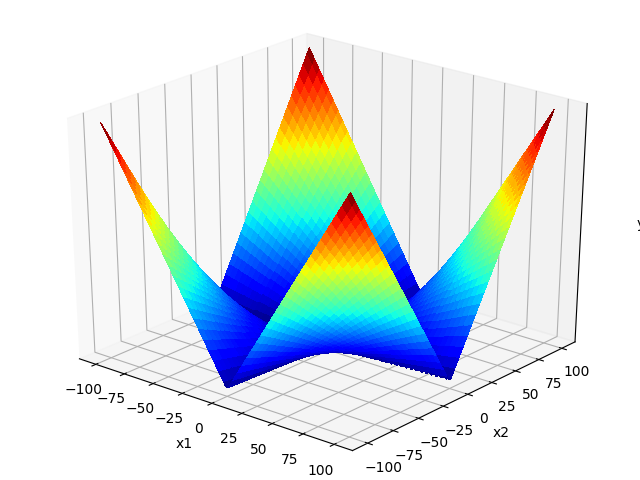
\includegraphics[width=1\linewidth]{png/functions/islo_uni_F4}
  	 \includegraphics[width=1\linewidth]{png/functions/islo_uni_F5}
  	 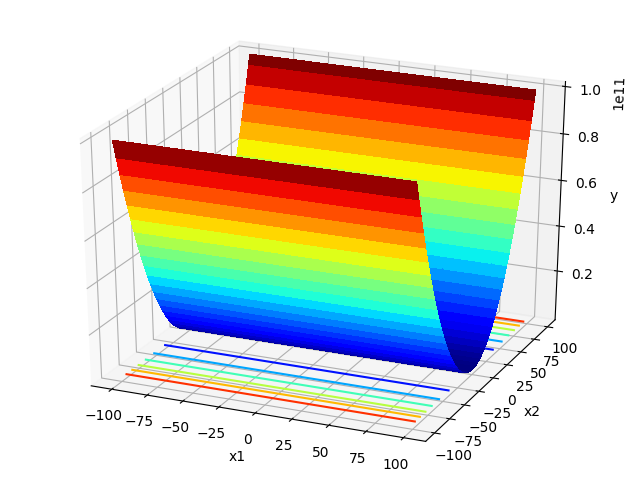
\includegraphics[width=1\linewidth]{png/functions/islo_uni_F7}
  	 \includegraphics[width=1\linewidth]{png/functions/islo_uni_F8}
  	\caption{Unimodal}
  	\label{subfig:uni}
  	\end{subfigure}
    \begin{subfigure}{0.24\textwidth}
   	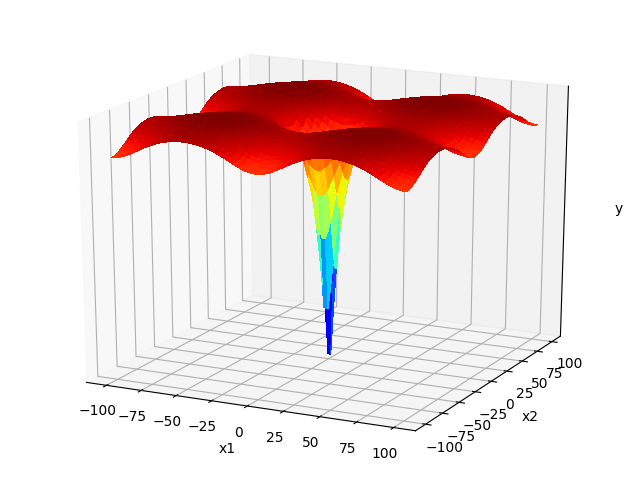
\includegraphics[width=1\linewidth]{png/functions/islo_multi_F9}
  	 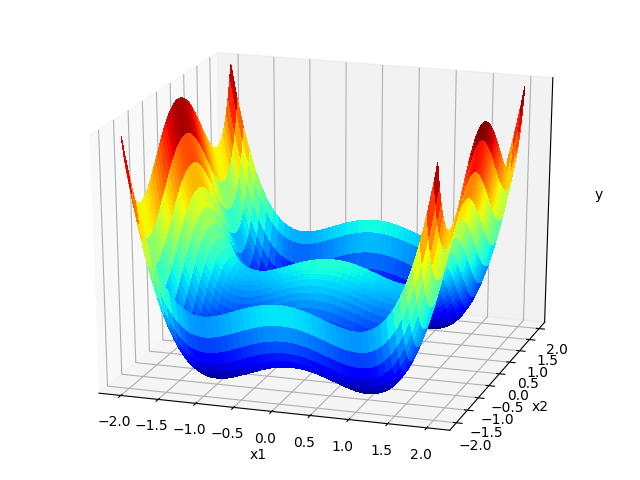
\includegraphics[width=1\linewidth]{png/functions/islo_multi_F11}
  	 \includegraphics[width=1\linewidth]{png/functions/islo_multi_F15}
  	 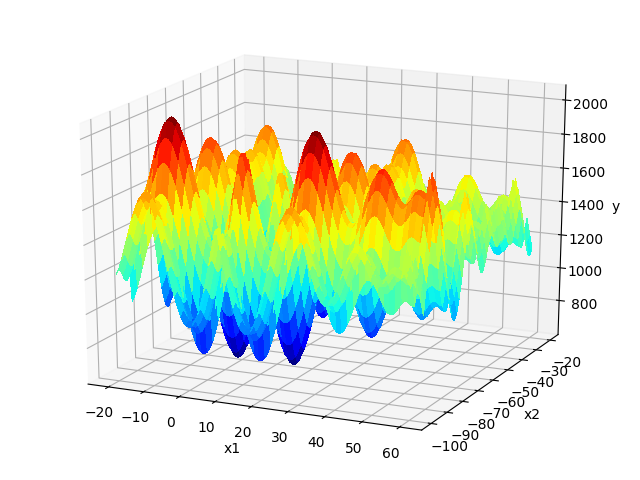
\includegraphics[width=1\linewidth]{png/functions/islo_multi_F16}
  	 \caption{Multimodal}
  	\label{subfig:multi}
  	\end{subfigure}
   \begin{subfigure}{0.24\textwidth}
   	\includegraphics[width=1\linewidth]{png/functions/islo_hybrid_F17}
  	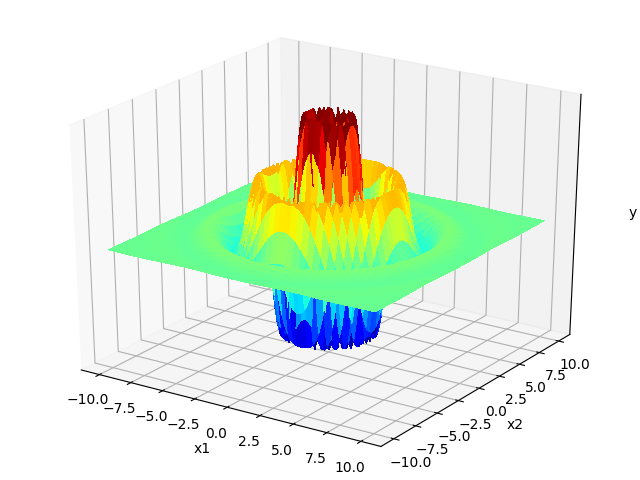
\includegraphics[width=1\linewidth]{png/functions/islo_hybrid_F19}
  	\includegraphics[width=1\linewidth]{png/functions/islo_hybrid_F21}
  	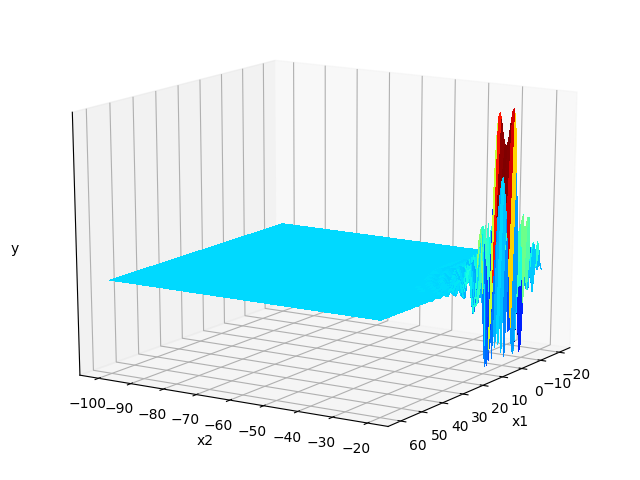
\includegraphics[width=1\linewidth]{png/functions/islo_hybrid_F22}
  	 \caption{Hybrid}
  	\label{subfig:hybrid}
  	\end{subfigure}
  	\begin{subfigure}{0.24\textwidth}
  	 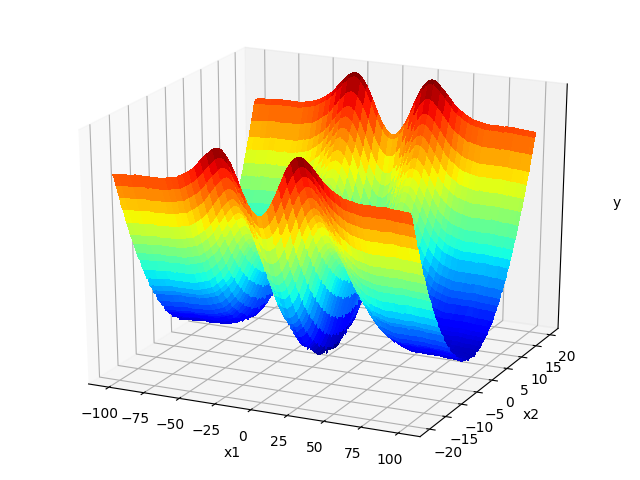
\includegraphics[width=1\linewidth]{png/functions/islo_compos_F26}
  	 \includegraphics[width=1\linewidth]{png/functions/islo_compos_F28}
  	 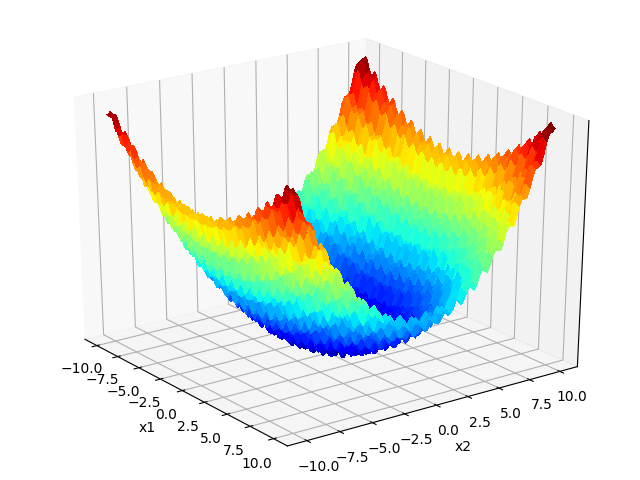
\includegraphics[width=1\linewidth]{png/functions/islo_compos_F29}
  	 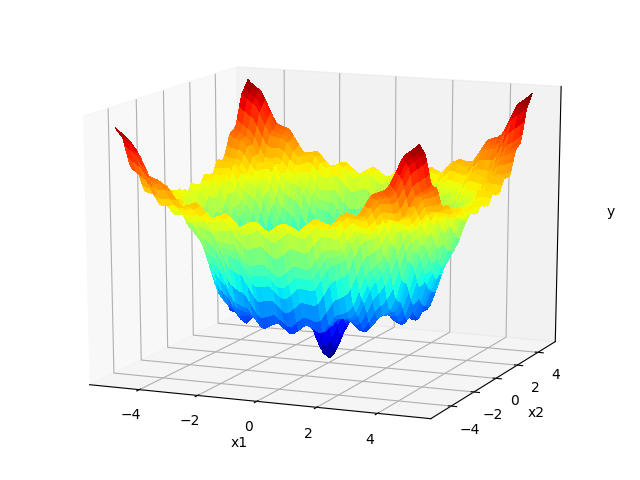
\includegraphics[width=1\linewidth]{png/functions/islo_compos_F30}
  	 \caption{Composition}
  	\label{subfig:compos}
  	\end{subfigure}
  \caption{Examples of 3D plot for each kind of benchmark functions.} 
  \label{fig_functions} 
\end{figure}

The detail such as name, formula, search space and optimal value of each function is shown in Table. [\ref{tbl_uni_funcs}-\ref{tbl_compos_funcs}]. Also, Fig. \ref{fig_functions} presents the typical 3D plots of the cost function for some test cases considered in this study. 

\begin{table}[!t]
\caption{Description of unimodal benchmark functions}
\label{tbl_uni_funcs}
\centering
\begin{tabular}{p{9cm} p{2cm} p{1cm}}
 \hline Mathematical Definition & Range & $f_{min}$  \\ 
 \hline
$f_1(x) = \sum_{i=1}^n x_i^2$ & [-500, 500] & 0 \\
$f_2(x) =  \sum_{i=1}^n |x_i|$ & [-500, 500] & 0 \\
$f_3(x) =  max_{i = 1, 2,...,n}|x_i|)$ & [-500, 500] & 0 \\
$f_4(x) =  \sum_{i=1}^n |x_i| + \prod_{i=1}^n |x_i|$  & [-500, 500] & 0 \\
$f_5(x) =  \sum_{i=1}^n ix_i^2$ & [-500, 500] & 0 \\
$f_6(x) =  \sum_{i=1}^{n-1} (x_i^2)^{x_{i+1}^2+1} + (x_{i+1}^2)^{x_{i}^2+1}$ & [-500, 500] & 0 \\
$f_7(x) =  \sum_{i=1}^n (10^6)^{\frac{x_i-1}{n-1}} + 100$ & [-500, 500] & 100 \\
$f_8(x) = x_1^2 + 10^6\sum_{i=2}^n x_i^2$ + 200 & [-500, 500] & 200 \\
 \hline
\end{tabular}
\end{table}

\begin{table}[!t]
\caption{Description of multimodal benchmark functions}
\label{tbl_multi_funcs}
\centering
\begin{tabular}{p{9cm} p{2cm} p{1cm}}
 \hline 
 Mathematical Definition & Range & $f_{min}$  \\ 
 \hline
$f_9(x) = -a.exp(-b\sqrt{\frac{1}{n}\sum_{i=1}^{n}x_i^2})-exp(\frac{1}{n}\sum_{i=1}^{n}cos(cx_i))+ a + exp(1)$ with a = 20 and b = 0.2 & [-500, 500] & 0 \\
$f_{10}(x) =\left[\left(||\textbf{x}||^2 - n\right)^2\right]^\alpha + \frac{1}{n}\left(\frac{1}{2}||\textbf{x}||^2+\sum_{i=1}^{n}x_i\right)+\frac{1}{2}$ & [-500, 500] & 0 \\
$f_{11}(x) =\sum_{i=1}^{n}(x^2-i)^2$ & [-500, 500] & 0 \\
$f_{12}(x)=1-cos(2\pi\sqrt{\sum_{i=1}^{D}x_i^2})+0.1\sqrt{\sum_{i=1}^{D}x_i^2}$ & [-500, 500] & 0 \\
$f_{13}f(x)=\sum_{i=1}^{n}[b (x_{i+1} - x_i^2)^ 2 + (a - x_i)^2]$ & [-500, 500] & 0 \\
$f_{14}(x) = \sum_{i=1}^{n}{\sum_{j=1}^5{j sin((j+1)x_i+j)} + 300}$ & [-500, 500] & 300 \\
$f_{15}(x)=10n + \sum_{i=1}^{n}(x_i^2 - 10cos(2\pi x_i)) + 400$ & [-500, 500] & 400 \\
$f_{16}(x) = 418.9829D -{\sum_{i=1}^{n} x_i sin(\sqrt{|x_i|})}. + 500$ & [-500, 500] & 500 \\
\hline
\end{tabular}
\end{table}

The performance of ISLO algorithm about optimizing 30 benchmark functions is compared with different optimizers including well-known algorithms as well as recent algorithms that belong to all four groups in nature-inspired meta-heuristic algorithms. Specifically, they are: 
\begin{itemize}
\item Generic Algorithm (GA) \cite{whitley1994genetic} (Evolutionary algorithms)
\item Particle Swarm Optimization (PSO) \cite{kennedy2010particle}, Whale Optimization Algorithm (WOA) \cite{mirjalili2016whale} and the original Sea Lion Optimization Algorithm (SLnO) \cite{masadeh2019sea} (Swarm-based algorithms)
\item Tug of War Optimization (TWO) \cite{kaveh2016novel} (Physics-based algorithms)
\item Queuing Search Optimization (QSO) \cite{zhang2018queuing} (Human-based algorithms)
\end{itemize}

\begin{table}[!t]
\caption{Description of hybrid benchmark functions}
\label{tbl_hybrid_funcs}
\centering
\begin{tabular}{p{9cm} p{2cm} p{1cm}}
 \hline Mathematical Definition & Range & $f_{min}$  \\ 
 \hline
$f_{17}$ (function 17 in CEC 2014) & \multirow{3}{*}{[-500, 500]} & \multirow{3}{*}{1700} \\
p = [0.3, 0.4, 0.3] & \\
Modified Schwefel's , Rastrigin's  and High Conditioned Elliptic Functions & \\ \hline
$f_{18}$ (function 18 in CEC 2014) & \multirow{3}{2cm}{[-500, 500]} & \multirow{3}{1cm}{1800} \\
p = [0.3, 0.4, 0.3] & \\
Bent Cigar, HGBat and Rastrigin’s Functions & \\ \hline
$f_{19}$ (function 19 in CEC 2014) & \multirow{3}{2cm}{[-500, 500]} & \multirow{3}{1cm}{1900} \\
p = [ 0.2, 0.2, 0.3, 0.3] & \\
Griewank’s, Weierstrass, Rosenbrock’s and Scaffer’s Functions & \\ \hline
$f_{20}$ (function 20 in CEC 2014) & \multirow{3}{2cm}{[-500, 500]} & \multirow{3}{1cm}{2000} \\
p =  [0.2, 0.2, 0.3, 0.3] & \\
HGBat , Discus, Expanded Griewank’s plus Rosenbrock’s  and Rastrigin’s Functions & \\ \hline
$f_{21}$ (function 6 in CEC 2015) & \multirow{3}{2cm}{[-500, 500]} & \multirow{3}{1cm}{600} \\
p =  [0.3,0.3,0.4]  & \\
Modified Schwefel's , Rastrigin's, High Conditioned Elliptic Functions & \\ \hline
$f_{22}$ (function 7 in CEC 2015) & \multirow{3}{2cm}{[-500, 500]} & \multirow{3}{1cm}{700} \\
p =[0.2,0.2,0.3,0.3]  & \\
Griewank's , Weierstrass ,Rosenbrock's and Scaffer's Functions & \\ \hline
$f_{23}$ (function 8 in CEC 2015) & \multirow{3}{2cm}{[-500, 500]} & \multirow{3}{1cm}{800} \\
p = [0.1,0.2,0.2,0.2,0.3]  & \\
Scaffer’s , HGBat ,Rosenbrock’s, Modified Schwefel’s and High Conditioned Elliptic Functions & \\ \hline
\end{tabular}
\end{table}

\begin{table}[!t]
\caption{Description of composition benchmark functions}
\label{tbl_compos_funcs}
\centering
\begin{tabular}{p{9cm} p{2cm} p{1cm}}
 \hline Mathematical Definition & Range & $f_{min}$  \\ 
 \hline
$f_{24}$ (function 9 in CEC 2015) & \multirow{4}{*}{[-500, 500]} & \multirow{3}{*}{900} \\
$\sigma = $ [20, 20, 20] & \\
$\lambda = $ [1, 1, 1] & \\
Schwefel's , Rastrigin's  and  HGBat  Functions & \\ \hline
$f_{25}$ (function 10 in CEC 2015) & \multirow{4}{*}{[-500, 500]} & \multirow{3}{*}{1000} \\
$\sigma = $  [10, 30,50]  & \\
$\lambda = $  [1, 1, 1]  & \\
$f_{21}$, $f_{22}$ and $f_{23}$ Functions & \\ \hline
$f_{26}$ (function 11 in CEC 2015) & \multirow{4}{*}{[-500, 500]} & \multirow{3}{*}{1100} \\
$\sigma = $  [10, 10, 10, 20, 20]  & \\
$\lambda = $  [10, 10, 2.5, 25,1e-6]  & \\
 HGBat ,  Rastrigin’s  and   Schwefel's,  Weierstrass and  High Conditioned Elliptic   Functions & \\ \hline
$f_{27}$ (function 12 in CEC 2015) & \multirow{4}{*}{[-500, 500]} & \multirow{3}{*}{1200} \\
$\sigma = $  [10,20,20,30,30] & \\
$\lambda = $ [0.25, 1, 1e-7, 10, 10]  & \\
 Schwefel's  , Rastrigin's  and   High Conditioned Elliptic, Expanded Scaffer’s and  HappyCat Functions & \\ \hline
$f_{28}$ (function 13 in CEC 2015) & \multirow{4}{*}{[-500, 500]} & \multirow{3}{*}{1300} \\
$\sigma = $  [10, 10, 10, 20, 20]  & \\
$\lambda = $  [1, 10, 1, 25, 10]  & \\
$f_{23}$ , Rastrigin's  and  $f_{21}$,  Schwefel's  and  Expanded Scaffer’s  Functions & \\ \hline
$f_{29}$ (function 14 in CEC 2015) & \multirow{4}{*}{[-500, 500]} & \multirow{3}{*}{1400} \\
$\sigma = $  [10, 20, 30, 40, 50, 50, 50] & \\
$\lambda = $  [10,2.5, 2.5, 10,1e-6,1e-6, 10] & \\
HappyCat , Griewank’s plus Rosenbrock’s, Schwefel's, Expanded Scaffer’s, High Conditioned Elliptic, Cigar and  and Rastrigin’s  Functions & \\ \hline
$f_{30}$ (function 15 in CEC 2015) & \multirow{4}{*}{[-500, 500]} & \multirow{3}{*}{1500} \\
$\sigma = $  [10, 10, 20, 20, 30, 30, 40, 40, 50, 50] & \\
$\lambda = $  [0.1,2.5e-1, 0.1, 2.5e-2, 1e-3, 0.1, 1e-5, 10, 2.5e-2, 1e-3] & \\
Rastrigin’s  , Weierstrass, HappyCat, Schwefel's, Rosenbrock's, HGBat, Katsuura, Expanded Scaffer’s, Expanded Griewank’s  and  Ackley  Functions & \\ \hline

\end{tabular}
\end{table}

\subsection{Evaluation method and Parameter settings}

	With compared algorithms and functions mentioned above, the experimental results of each model are produced by calculating mean and standard deviation ($std$) value (Eq. \ref{eq_mean} and \ref{eq_std}) of 20 times running starting from randomly generated populations for each algorithms. For all the algorithms, a population size and maximum iteration equal to 100 and 500 have been utilized to run on each function with 50-dimension search space. The choices  of parameters are based on existing setting up
described in original paper of each algorithm.
\begin{equation} \label{eq_mean}
mean = \frac{1}{n}\sum_{i=1}^n r_i
\end{equation}
\begin{equation}\label{eq_std}
std = \sqrt{\frac{1}{n-1}\sum_{i=1}^n(r_i - r)^2}
\end{equation}
where $N$ is the number of values and $r_i$ $(i = 1, 2, ..., N)$ are observations.
	
	For each function, after calculating $mean$ and $std$ values of each algorithm, the best results will be highlighted in both. The best results are determined by following rules:
\begin{itemize}
\item $mean$ values are considered at first. If in a case, an algorithm own the best $mean$ value, it will be ranked as the best optimizer.
\item In the case where there are two or more algorithms having the same $mean$ value, the one that has the most stable $std$ value will be chosen as the best one.
\end{itemize}
	
	Finally, the experimental results of all functions and algorithms are shown in Table \ref{tbl_results_uni_multi} and \ref{tbl_results_hybrid_compos}, and the convergence speeds of the algorithms in several functions are illustrated in Fig. \ref{fig_uni_multi_convergence} and \ref{fig_hybrid_compos_convergence}.

\begin{table}[!t]
\caption{Comparison of optimization results obtained for the unimodal and multimodal functions}
\label{tbl_results_uni_multi}
\centering
\resizebox{\textwidth}{!}{%
\begin{tabular}{|l|l|l|l|l|l|l|l|l|}
\hline
Function             &      & GA       & PSO      & SLnO     & WOA               & ISLO               & TWO      & QSO               \\ \hline
\multirow{3}{*}{$f_1$}  & mean & 4.64E+01 & 9.69E+02 & 2.52E-25 & 2.26E-80          & \textbf{3.26E-120} & 1.06E+01 & 8.14E-01          \\ \cline{2-9} 
                     & std  & 7.54E+00 & 3.12E+02 & 7.11E-25 & 9.41E-80          & \textbf{8.45E-120} & 1.39E+00 & 3.08E-01          \\ \cline{2-9} 
                     & rank & 6        & 7        & 3        & 2                 & \textbf{1}         & 5        & 4                 \\ \hline
\multirow{3}{*}{$f_2$}  & mean & 2.19E+02 & 1.99E+02 & 1.64E+01 & 2.98E+00          & \textbf{2.26E-01}  & 2.49E+01 & 2.62E+00          \\ \cline{2-9} 
                     & std  & 1.44E+01 & 3.42E+01 & 2.38E+00 & 5.86E-01          & \textbf{1.23E-01}  & 2.24E+00 & 6.15E-01          \\ \cline{2-9} 
                     & rank & 7        & 6        & 4        & 3                 & \textbf{1}         & 5        & 2                 \\ \hline
\multirow{3}{*}{$f_3$}  & mean & 4.30E+00 & 1.79E+01 & 7.58E+01 & 4.39E+01          & \textbf{6.25E-58}  & 1.58E+01 & 1.82E+01          \\ \cline{2-9} 
                     & std  & 1.11E+00 & 2.28E+00 & 1.92E+01 & 2.29E+01          & \textbf{2.64E-57}  & 3.93E+00 & 1.43E+00          \\ \cline{2-9} 
                     & rank & 2        & 4        & 7        & 6                 & \textbf{1}         & 3        & 5                 \\ \hline
\multirow{3}{*}{$f_4$}  & mean & 1.12E+02 & 7.43E+02 & 4.07E+26 & 2.81E+00          & \textbf{1.56E-01}  & 1.71E+32 & 1.79E+02          \\ \cline{2-9} 
                     & std  & 7.57E+00 & 1.22E+02 & 1.30E+27 & 7.00E-01          & \textbf{1.01E-01}  & 7.33E+32 & 1.98E+02          \\ \cline{2-9} 
                     & rank & 3        & 5        & 6        & 2                 & \textbf{1}         & 7        & 4                 \\ \hline
\multirow{3}{*}{$f_5$}  & mean & 1.36E+03 & 1.58E+04 & 2.01E+02 & 2.42E+00          & \textbf{3.52E-02}  & 2.24E+03 & 2.43E+01          \\ \cline{2-9} 
                     & std  & 3.87E+02 & 5.57E+03 & 9.51E+01 & 6.70E-01          & \textbf{6.06E-02}  & 1.06E+03 & 1.20E+01          \\ \cline{2-9} 
                     & rank & 5        & 7        & 4        & 2                 & \textbf{1}         & 6        & 3                 \\ \hline
\multirow{3}{*}{$f_6$}  & mean & 1.27E+00 & 1.20E+00 & 3.27E-01 & 4.71E-03          & \textbf{5.65E-05}  & 1.02E+00 & 7.83E-02          \\ \cline{2-9} 
                     & std  & 3.01E-02 & 4.08E-02 & 1.47E-01 & 1.40E-03          & \textbf{5.50E-05}  & 2.21E-02 & 4.22E-02          \\ \cline{2-9} 
                     & rank & 7        & 6        & 4        & 2                 & \textbf{1}         & 5        & 3                 \\ \hline
\multirow{3}{*}{$f_7$}  & mean & 8.70E+06 & 2.34E+07 & 1.42E+06 & 6.12E+04          & \textbf{8.22E+02}  & 1.22E+08 & 1.27E+04          \\ \cline{2-9} 
                     & std  & 2.66E+06 & 1.17E+07 & 1.12E+06 & 2.05E+04          & \textbf{1.10E+02}  & 4.97E+07 & 5.12E+03          \\ \cline{2-9} 
                     & rank & 5        & 6        & 4        & 3                 & \textbf{1}         & 7        & 2                 \\ \hline
\multirow{3}{*}{$f_8$}  & mean & 4.54E+08 & 7.70E+09 & 6.52E+07 & 7.83E+05          & \textbf{1.60E+04}  & 1.02E+08 & 8.19E+06          \\ \cline{2-9} 
                     & std  & 1.10E+08 & 2.70E+09 & 2.65E+07 & 2.47E+05          & \textbf{1.20E+04}  & 1.42E+07 & 3.40E+06          \\ \cline{2-9} 
                     & rank & 6        & 7        & 4        & 2                 & \textbf{1}         & 5        & 3                 \\ \hline
                     \multirow{3}{*}{$f_9$}  & mean & 1.69E+01 & 2.04E+01 & 2.05E+01 & 2.82E-01          & \textbf{1.85E-02}  & 2.01E+01 & 2.08E+01          \\ \cline{2-9} 
                     & std  & 3.02E-01 & 8.70E-01 & 3.00E-01 & 2.22E-01          & \textbf{1.11E-02}  & 3.89E-02 & 2.81E-02          \\ \cline{2-9} 
                     & rank & 3        & 5        & 6        & 2                 & \textbf{1}         & 4        & 7                 \\ \hline
\multirow{3}{*}{$f_{10}$} & mean & 6.71E+00 & 1.42E+01 & 3.55E-01 & 3.41E-01          & \textbf{4.34E-04}  & 7.68E-01 & 7.05E-01          \\ \cline{2-9} 
                     & std  & 9.85E-01 & 3.00E+00 & 8.31E-02 & 1.35E-01          & \textbf{1.89E-03}  & 1.25E-01 & 6.88E-02          \\ \cline{2-9} 
                     & rank & 6        & 7        & 3        & 2                 & \textbf{1}         & 5        & 4                 \\ \hline
\multirow{3}{*}{$f_{11}$} & mean & 2.11E+04 & 2.99E+04 & 5.25E+03 & \textbf{3.14E+03} & 9.01E+03           & 5.20E+03 & 6.09E+03          \\ \cline{2-9} 
                     & std  & 2.43E+03 & 1.50E+04 & 3.25E+03 & \textbf{1.42E+03} & 5.01E+02           & 1.77E+03 & 7.24E+02          \\ \cline{2-9} 
                     & rank & 6        & 7        & 3        & \textbf{1}        & 5                  & 2        & 4                 \\ \hline
\multirow{3}{*}{$f_{12}$} & mean & 3.84E+00 & 5.30E+00 & 7.25E-01 & 3.75E-01          & \textbf{9.50E-02}  & 1.76E+00 & 1.87E+00          \\ \cline{2-9} 
                     & std  & 3.09E-01 & 5.25E-01 & 6.98E-02 & 9.94E-02          & \textbf{2.00E-02}  & 3.93E-01 & 2.05E-01          \\ \cline{2-9} 
                     & rank & 6        & 7        & 3        & 2                 & \textbf{1}         & 4        & 5                 \\ \hline
\multirow{3}{*}{$f_{13}$} & mean & 8.18E+04 & 4.77E+06 & 1.45E+03 & 5.63E+01          & \textbf{3.85E-01}  & 5.40E+04 & 6.70E+03          \\ \cline{2-9} 
                     & std  & 1.97E+04 & 2.83E+06 & 5.67E+02 & 2.75E+00          & \textbf{3.67E-01}  & 9.53E+04 & 4.26E+03          \\ \cline{2-9} 
                     & rank & 6        & 7        & 3        & 2                 & \textbf{1}         & 5        & 4                 \\ \hline
\multirow{3}{*}{$f_{14}$} & mean & 3.17E+02 & 3.20E+02 & 3.21E+02 & 3.00E+02          & \textbf{3.00E+02}  & 3.20E+02 & 3.21E+02          \\ \cline{2-9} 
                     & std  & 3.42E-01 & 7.51E-01 & 2.93E-01 & 1.92E-01          & \textbf{1.37E-02}  & 3.78E-02 & 2.91E-02          \\ \cline{2-9} 
                     & rank & 3        & 5        & 7        & 2                 & \textbf{1}         & 4        & 6                 \\ \hline
\multirow{3}{*}{$f_{15}$} & mean & 2.75E+04 & 7.21E+04 & 4.21E+03 & 5.42E+02          & \textbf{4.02E+02}  & 3.17E+05 & 4.46E+02          \\ \cline{2-9} 
                     & std  & 9.46E+03 & 3.66E+04 & 2.29E+03 & 5.50E+01          & \textbf{2.43E+00}  & 1.28E+05 & 3.07E+01          \\ \cline{2-9} 
                     & rank & 5        & 6        & 4        & 3                 & \textbf{1}         & 7        & 2                 \\ \hline
\multirow{3}{*}{$f_{16}$} & mean & 5.21E+02 & 5.21E+02 & 5.21E+02 & 5.03E+02          & \textbf{5.00E+02}  & 5.20E+02 & 5.21E+02          \\ \cline{2-9} 
                     & std  & 4.48E-02 & 1.66E-01 & 1.75E-01 & 5.94E+00          & \textbf{3.80E-01}  & 3.76E-02 & 1.99E-02          \\ \cline{2-9} 
                     & rank & 5        & 6        & 7        & 2                 & \textbf{1}         & 3        & 4                 \\ \hline
\end{tabular}%
}
\end{table}
	
\subsection{Experiment results and discussion}
\label{exp_results}

\subsubsection{Unimodal and Multimodal benchmark functions}
\begin{figure}[!ht] 
   \centering
   \begin{subfigure}{0.49\textwidth}
   	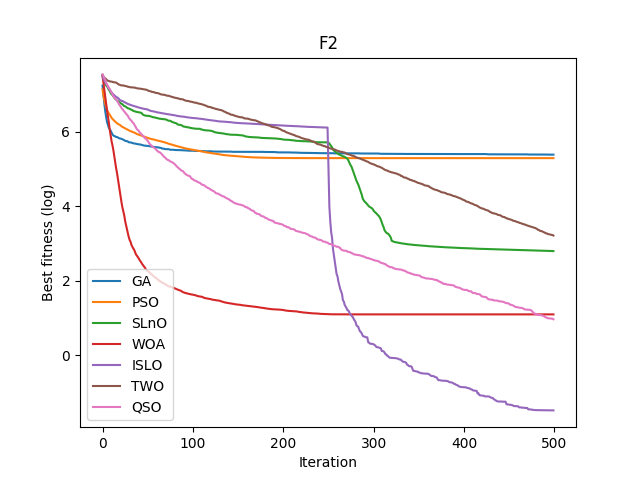
\includegraphics[width=1\linewidth]{png/convergence/islo_uni_F2}
  	 \includegraphics[width=1\linewidth]{png/convergence/islo_uni_F5}
  	 \includegraphics[width=1\linewidth]{png/convergence/islo_uni_F8}
  	\caption{Unimodal}
  	\label{subfig:uni_convergence}
  	\end{subfigure}
   \begin{subfigure}{0.49\textwidth}
   	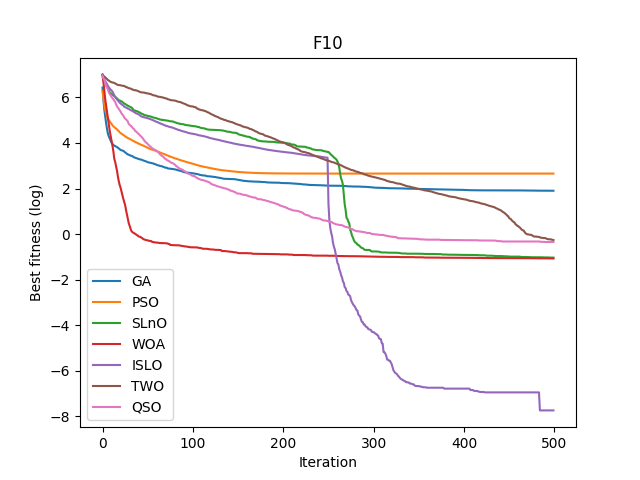
\includegraphics[width=1\linewidth]{png/convergence/islo_multi_F10}
  	 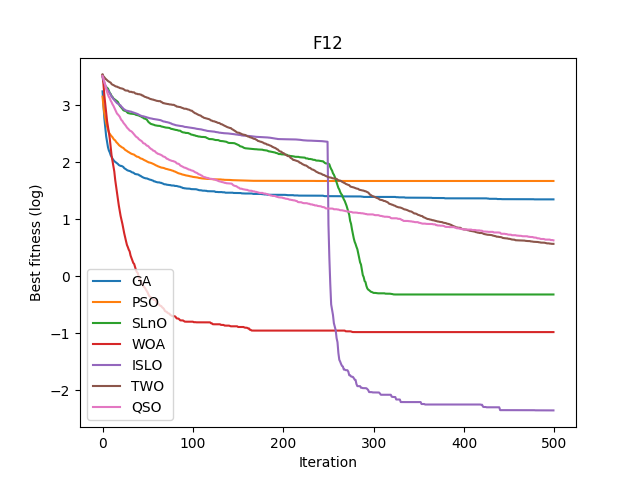
\includegraphics[width=1\linewidth]{png/convergence/islo_multi_F12}
  	 \includegraphics[width=1\linewidth]{png/convergence/islo_multi_F15}
  	 \caption{Multimodal}
  	\label{subfig:multi_convergence}
  	\end{subfigure}
  \caption{Convergence speed of each algorithm on unimodal (a) and multimodal (b) functions.} 
  \label{fig_uni_multi_convergence} 
\end{figure}
	Functions $f_1$ - $f_{16}$ are unimodal and multimodal functions. These kinds of functions are selected following a couple of testing purposes. Specifically, unimodal functions allow us to evaluate exploitation performance of meta-heuristic optimizers since they only have one global optimal minimum; multimodal functions help us see algorithms' exploration performance with a number of local minimum points, which exponentially increases following the increase in search space dimension. In general, it can be seen from the Table \ref{tbl_results_uni_multi} that ISLO shows the best performance among all chosen algorithms in the most test cases except $f_{11}$. Furthermore, while optimizing several functions, ISLO is able to reach or nearly the optimal value with decent stability.
	 
	\textbf{The accuracy and the stability:} From the gained results of unimodal and multimodal funtions in Table. \ref{tbl_results_uni_multi}, it could be made the following observations:
\begin{itemize}
\item ISLO outperforms the others in all test cases except $f_{11}$. In the experiments with unimodal functions $f_1$-$f_8$, ISLO is the best algorithm in the term of exploitation ability, being ranked at the first position among all chosen algorithms. The results with functions $f_1$ and $f_3$ indicate that ISLO could lead the population relatively near the global optimal position. Additionally, along with the best results in term of accuracy, ISLO also performs good stability since the standard deviation values are below 1 in all cases, especially in $f_1$ and $f_3$, the $std$ values are mostly 0. The results prove that compared with the original SLnO, ISLO's exploitation ability is significantly enhanced. 
\item The results in Table. \ref{tbl_results_uni_multi} for multimodal functions $f_9$-$f_{16}$ indicate that ISLO also has a superior exploration ability. ISLO stands at the first ranking in 7 out of 8 functions, and with $f_{14}$ and $f_{16}$ ISLO reaches the global optimal values of the functions, accompanying with that is relatively small standard deviation values. It is notable that ISLO is less competitive at $f_{11}$ where it stands at $5th$ position, being outperformed by WOA, TWO and original SLnO. However, in $f_8$, $f_9$, $f_{10}$, $f_{13}$, $f_{14}$ and $f_{16}$, ISLO's results are much better than the others in both terms of accuracy and stability.
\end{itemize}
In summary, all gained results with unimodal and multimodal funtions figure out that ISLO has the excellent exploitation and exploration ability. This is due to the fact that apart from considering and updating search agents' position following the best agent, taking the best experience of each agent into account (Eq. \ref{islo_eq3}) helps ISLO exploits population's information far better than SLnO. Apart from this, opposition-based updating operation in the exploration phase enrichs the diversity of population, helping ISLO easily jumps out of local minimums.

	\textbf{The convergence speed:} The convergence speed of all algorithms working on several functions are shown in Fig. \ref{fig_uni_multi_convergence}. It is clear that ISLO always considerably enhance its global best fitness values in the second half of the iterations. The reason is that on the first half of th e iterations, ISLO is in its exploration phase (since the value of C during that time is always greater than 1, see Algorithm \ref{algorithm_islo}). After changing to exploitation phase, ISLO has the ability to exploit and converge to global minimum quickly, providing better results than the others. Fig. \ref{fig_uni_multi_convergence} indicates that ISLO is competitive with an acceptable convergence speed, and also providing decent fitness values in functions $f_2$, $f_5$, $f_8$, $f_{10}$, $f_{12} $ and $f_{15}$. SLnO has the same pattern of convergence curves compared with ISLO, but it coverges to mediocre fitness values, especially in $f_2$, $f_5$ and $f_{10}$. Also, WOA and QSO are competitive compared with ISLO in function $f_{15}$, where the final results of them are extremely close to ISLO's.
	
\begin{table}[!t]
\caption{Comparison of optimization results obtained for the hybrid and composition benchmark functions}
\label{tbl_results_hybrid_compos}
\centering
\resizebox{\textwidth}{!}{%
\begin{tabular}{|l|l|l|l|l|l|l|l|l|}
\hline
Function             &      & GA       & PSO      & SLnO     & WOA               & ISLO               & TWO      & QSO               \\ \hline
\multirow{3}{*}{$f_{17}$} & mean & 2.19E+05 & 1.46E+05 & 8.08E+04 & 8.82E+03          & \textbf{1.81E+03}  & 2.08E+06 & 5.46E+03          \\ \cline{2-9} 
                     & std  & 1.29E+05 & 7.68E+04 & 4.92E+04 & 2.63E+03          & \textbf{1.95E+02}  & 7.79E+05 & 5.00E+02          \\ \cline{2-9} 
                     & rank & 6        & 5        & 4        & 3                 & \textbf{1}         & 7        & 2                 \\ \hline
\multirow{3}{*}{$f_{18}$} & mean & 6.43E+06 & 3.15E+04 & 9.29E+05 & 8.12E+03          & 4.46E+03           & 4.73E+05 & \textbf{3.49E+03} \\ \cline{2-9} 
                     & std  & 1.10E+06 & 9.41E+03 & 1.66E+06 & 2.55E+03          & 2.95E+03           & 1.00E+05 & \textbf{8.92E+02} \\ \cline{2-9} 
                     & rank & 7        & 4        & 6        & 3                 & 2                  & 5        & \textbf{1}        \\ \hline
\multirow{3}{*}{$f_{19}$} & mean & 8.97E+03 & 2.36E+03 & 2.48E+03 & 1.95E+03          & \textbf{1.92E+03}  & 9.67E+03 & 2.01E+03          \\ \cline{2-9} 
                     & std  & 2.87E+03 & 9.31E+02 & 8.36E+02 & 4.45E+01          & \textbf{2.08E+00}  & 2.02E+04 & 1.25E+02          \\ \cline{2-9} 
                     & rank & 6        & 4        & 5        & 2                 & \textbf{1}         & 7        & 3                 \\ \hline
\multirow{3}{*}{$f_{20}$} & mean & 1.82E+05 & 2.52E+04 & 1.49E+04 & 2.81E+03          & \textbf{2.12E+03}  & 4.53E+05 & 1.77E+04          \\ \cline{2-9} 
                     & std  & 2.14E+05 & 1.24E+04 & 6.90E+03 & 6.75E+02          & \textbf{8.47E+01}  & 1.03E+06 & 5.70E+04          \\ \cline{2-9} 
                     & rank & 6        & 5        & 3        & 2                 & \textbf{1}         & 7        & 4                 \\ \hline
\multirow{3}{*}{$f_{21}$} & mean & 7.97E+06 & 5.51E+07 & 1.04E+08 & 2.00E+05          & \textbf{3.19E+03}  & 1.79E+08 & 4.43E+08          \\ \cline{2-9} 
                     & std  & 2.95E+06 & 3.76E+07 & 1.00E+08 & 4.37E+05          & \textbf{9.01E+03}  & 8.02E+07 & 1.46E+08          \\ \cline{2-9} 
                     & rank & 3        & 4        & 5        & 2                 & \textbf{1}         & 6        & 7                 \\ \hline
\multirow{3}{*}{$f_{22}$} & mean & 2.28E+05 & 1.26E+07 & 1.85E+08 & 8.72E+02          & \textbf{7.16E+02}  & 1.17E+08 & 2.57E+08          \\ \cline{2-9} 
                     & std  & 7.52E+04 & 1.27E+07 & 6.11E+08 & 2.55E+02          & \textbf{9.38E-01}  & 1.29E+08 & 1.73E+08          \\ \cline{2-9} 
                     & rank & 3        & 4        & 6        & 2                 & \textbf{1}         & 5        & 7                 \\ \hline
\multirow{3}{*}{$f_{23}$} & mean & 5.29E+06 & 6.08E+07 & 2.65E+08 & 3.59E+04          & \textbf{1.26E+03}  & 2.74E+08 & 9.76E+08          \\ \cline{2-9} 
                     & std  & 1.29E+06 & 2.72E+07 & 3.12E+08 & 4.30E+04          & \textbf{1.19E+03}  & 1.57E+08 & 4.46E+08          \\ \cline{2-9} 
                     & rank & 3        & 4        & 5        & 2                 & \textbf{1}         & 6        & 7                 \\ \hline
                     \multirow{3}{*}{$f_{24}$} & mean & 1.12E+04 & 2.96E+04 & 3.46E+03 & 1.92E+03          & \textbf{1.81E+03}  & 1.15E+05 & 2.23E+03          \\ \cline{2-9} 
                     & std  & 2.35E+03 & 1.71E+04 & 1.04E+03 & 4.11E+01          & \textbf{1.62E+00}  & 4.71E+04 & 6.89E+02          \\ \cline{2-9} 
                     & rank & 5        & 6        & 4        & 2                 & \textbf{1}         & 7        & 3                 \\ \hline
\multirow{3}{*}{$f_{25}$} & mean & 8.17E+06 & 1.26E+08 & 8.62E+08 & 1.23E+05          & \textbf{2.95E+03}  & 2.64E+08 & 6.98E+08          \\ \cline{2-9} 
                     & std  & 2.42E+06 & 5.10E+07 & 1.08E+09 & 1.15E+05          & \textbf{4.98E+02}  & 1.09E+08 & 3.18E+08          \\ \cline{2-9} 
                     & rank & 3        & 4        & 7        & 2                 & \textbf{1}         & 5        & 6                 \\ \hline
\multirow{3}{*}{$f_{26}$} & mean & 6.78E+03 & 4.50E+03 & 4.63E+03 & 3.03E+03          & \textbf{2.22E+03}  & 4.20E+03 & 2.82E+03          \\ \cline{2-9} 
                     & std  & 3.59E+02 & 3.76E+02 & 9.84E+02 & 9.60E+02          & \textbf{2.03E+00}  & 2.15E+02 & 3.59E+01          \\ \cline{2-9} 
                     & rank & 7        & 5        & 6        & 3                 & \textbf{1}         & 4        & 2                 \\ \hline
\multirow{3}{*}{$f_{27}$} & mean & 3.22E+03 & 3.15E+03 & 2.52E+03 & 2.43E+03          & \textbf{2.40E+03}  & 2.87E+03 & 2.66E+03          \\ \cline{2-9} 
                     & std  & 6.09E+01 & 1.18E+02 & 1.66E-02 & 3.28E+00          & \textbf{1.50E+00}  & 2.58E+01 & 6.04E+00          \\ \cline{2-9} 
                     & rank & 7        & 6        & 3        & 2                 & \textbf{1}         & 5        & 4                 \\ \hline
\multirow{3}{*}{$f_{28}$} & mean & 2.11E+05 & 5.47E+04 & 1.06E+05 & 9.88E+04          & 8.02E+04           & 1.49E+05 & \textbf{3.25E+03} \\ \cline{2-9} 
                     & std  & 6.99E+03 & 1.22E+04 & 5.84E+03 & 7.98E+03          & 3.86E+04           & 3.89E+03 & \textbf{1.81E+00} \\ \cline{2-9} 
                     & rank & 7        & 2        & 5        & 4                 & 3                  & 6        & \textbf{1}        \\ \hline
\multirow{3}{*}{$f_{29}$} & mean & 3.77E+05 & 1.13E+07 & 2.17E+13 & 2.92E+03          & \textbf{2.83E+03}  & 2.39E+13 & 8.72E+06          \\ \cline{2-9} 
                     & std  & 2.07E+05 & 1.10E+05 & 1.27E+11 & 4.78E+01          & \textbf{5.36E+00}  & 3.05E+11 & 1.90E+06          \\ \cline{2-9} 
                     & rank & 3        & 5        & 6        & 2                 & \textbf{1}         & 7        & 4                 \\ \hline
\multirow{3}{*}{$f_{30}$} & mean & 4.31E+03 & 1.68E+06 & 3.04E+03 & 2.93E+03          & \textbf{2.91E+03}  & 1.12E+04 & 3.21E+03          \\ \cline{2-9} 
                     & std  & 7.28E+02 & 1.94E+06 & 5.60E-01 & 2.30E+00          & \textbf{1.32E+00}  & 1.54E+04 & 1.66E+02          \\ \cline{2-9} 
                     & rank & 5        & 7        & 3        & 2                 & \textbf{1}         & 6        & 4                 \\ \hline
\end{tabular}%
}
\end{table}

\begin{figure}[!ht] 
   \centering
   \begin{subfigure}{0.49\textwidth}
   	\includegraphics[width=1\linewidth]{png/convergence/islo_hybrid_F17}
  	 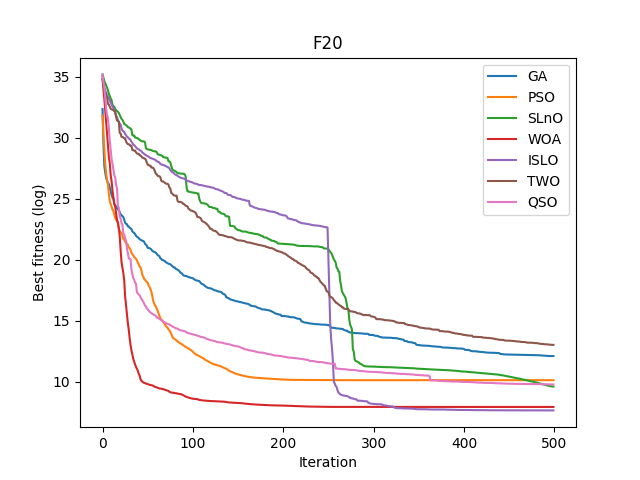
\includegraphics[width=1\linewidth]{png/convergence/islo_hybrid_F20}
  	 \includegraphics[width=1\linewidth]{png/convergence/islo_hybrid_F21}
  	\caption{Hybrid}
  	\label{subfig:hybrid_convergence}
  	\end{subfigure}
   \begin{subfigure}{0.49\textwidth}
   	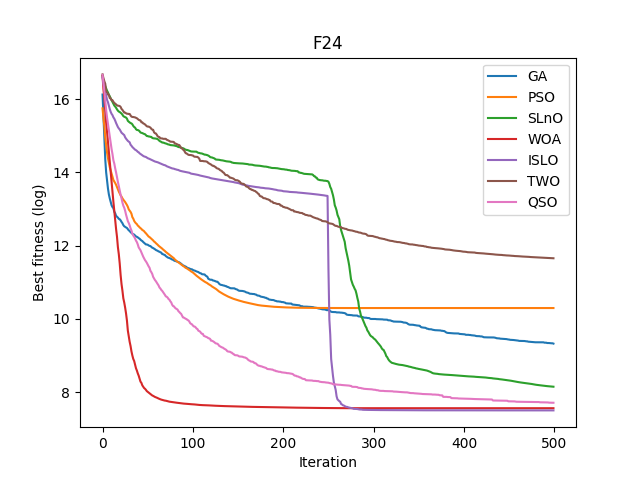
\includegraphics[width=1\linewidth]{png/convergence/islo_compos_F24}
  	 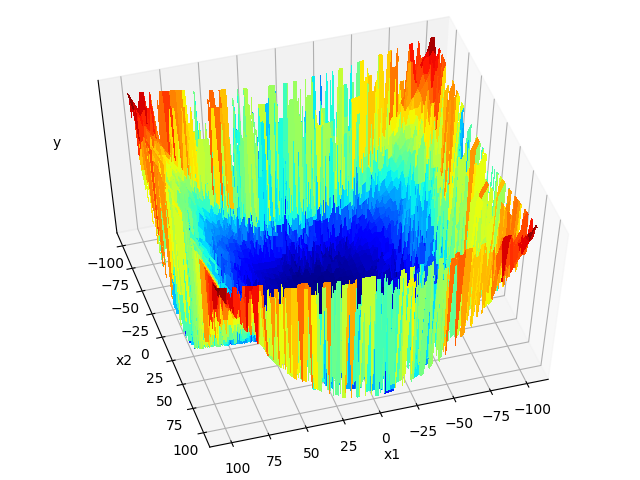
\includegraphics[width=1\linewidth]{png/convergence/islo_compos_F25}
  	 \includegraphics[width=1\linewidth]{png/convergence/islo_compos_F28}
  	 \caption{Composition}
  	\label{subfig:compos_convergence}
  	\end{subfigure}
  \caption{Convergence speed of each algorithm on hybrid (a) and composition (b) functions.} 
  \label{fig_hybrid_compos_convergence} 
\end{figure}
\subsubsection{Hybrid and Composition benchmark functions}

	Functions $f_{17}$-$f_{30}$ are hybrid and composition functions. In hybrid functions ($f_{17}$-$f_{23}$, the variables are randomly divided into subcomponents which play a role as input for different basic functions including both unimodal and multimodal functions. In order to work well on these functions, algorithms are required to be good at both exploitation and exploration capability, because hybrid functions are both unimodal and multimodal, and they own different properties for different variables subcomponents. On the other hand, optimization of composite mathematical functions ($f_{24}$-$f_{30}$) is a very challenging task, because local optima is only avoided by a proper balance between exploitation and exploration. In general, Fig. \ref{tbl_results_hybrid_compos} shows that ISLO owns the best performance over all hybrid and compostion functions. The results from ISLO stand at first ranking in all cases except $f_8$ and $f_{28}$ where the first position belongs to QSO. Also, as what is observed in Fig. \ref{fig_hybrid_compos_convergence}, ISLO's convergence curves are similar to those in unimodal and multimodal functions, and ISLO still has a very fast convergence after the first half of iteration because of its updating mechanism.
	

	
	\textbf{The accuracy and the stability:} 
	
	To resolve the optimization problem in hybrid functions $f_{17}$-$f_{23}$, it is evident that ISLO can work very well in almost cases. The results shown in Table. \ref{tbl_results_hybrid_compos} indicates that ISLO has the superior results at functions $f_{17}$, $f_{19}$, $f_{20}$ and $f_{23}$ compared with state-of-the-art algorithms such as WOA and QSO. Furthermore, with functions $f_{21}$ and $f_{23}$, ISLO's results are much better than the others', proving decent performance at both exploitation and exploration. Solving the case $f_{18}$, although ISLO does not account for the first place, it is still very competitive when its result is only worse than QSO's.
	
	For composition functions, ISLO shows the best performance among all the algorithms by standing at the first place in 6 out of 7 functions. Specifically, in $f_{24}$, $f_{27}$, $f_{29}$ and $f_{30}$, there is no big differences between ISLO'results and the others', while in $f_{25}$ and $f_{26}$, $mean$ and $std$ values from Table. \ref{tbl_results_hybrid_compos} indicates the dominance of ISLO in optimizing these functions. This proves that ISLO owns a superior balance between its exploitation and exploration while solving test problems. Also $std$ values from ISLO in most cases are below 10, showing the decent stability of this algorithm compared with GA or PSO algorithms.
	
	\textbf{The convergence speed:} As working on unimodal and multimodal functions, when working on hybrid and composite mathematical functions, ISLO still owns the fast convergence in the second half of iterations. The convergence curves in Fig. \ref{fig_hybrid_compos_convergence} shows that ISLO starts to converge very fast right after exploration phase comes to an end. In $f_{17}$ and $f_{24}$, the convergence curves indicate that ISLO is very competitive with WOA because these 2 algorithm converge to almost one value. Also, the results comes from ISLO is far better than the original SLnO in all cases, proving that exploitation and exploration capacities in SLnO are considerably enhanced. QSO is observed to be superior in function $f_{28}$, in which the others including ISLO are stuck in local minimums.   

\section{Application}
\label{sec:exp_app}
	
	In this section, proposed model in Section \ref{sec:application} is utilized for solving time-series prediction in the auto-scaling problem in cloud computing. Our experiment is done with 4 datasets: Google Trace CPU, Google Trace Memory, EU Internet Traffic and UK Internet Traffic. In this empirical study, ISLO-CFNN model is compared with several deep learning models such as simple MLP, the original CFNN, the original RNN and two well-known and widely used models in time-series forecasting: LSTM and GRU in terms of accuracy and run time. Also, optimizing capability of ISLO on CFNN is compared with several swarm-based algorithms in Section \ref{sec:exp_theory}. The bio-inspired models used to validate against ISLO-CFNN are PSO-CFNN and SLnO-CFNN, which are CFNN models optimized by PSO and SLnO algorithms, respectively.
	
	We would first describe 4 datasets used in this experiment. Then, the parameter setting for each model and evaluation metrics are introduced in detail. Finally, ISLO-CFNN performance is compared with the deep learning models as well as bio-inspired models in different perspectives.

\subsection{Dataset and Set up}
\label{exp:data}

\subsubsection{Google Trace dataset}
	The most important dataset in our experiments is gathered by Google on a cluster of about $12500$ machines \cite{reiss2011google} during 29 days, starting from May 2011. Resources requirement and usage data for each jobs are recorded by each machine in cluster, and then the data is managed by cluster's management system. In Google Trace dataset, there are two important columns, which are about two extremely important information of Central Processing Unit (CPU) and Random Access Memory (RAM) required for each job. For that reason, we decide to choose these two information as two time-series datasets (called Google Trace CPU and Google Trace RAM from here). The datasets are processed and summarized in 5-minute interval, containing 8351 data points, and considered as the total demand for resources in the whole Google's cluster. Visualization of Google Trace CPU and Google Trace RAM datasets is illustrated in Fig. \ref{fig_data_ggtrace}. 
	
\begin{figure}[!ht] 
   \centering
   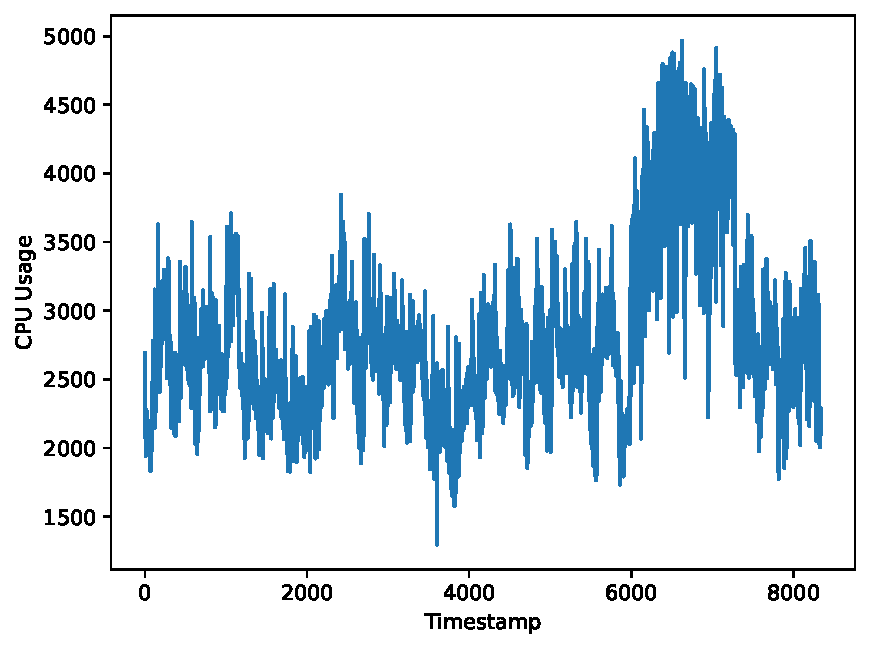
\includegraphics[width=0.49\linewidth]{/pdf/dataset/cpu_full}
   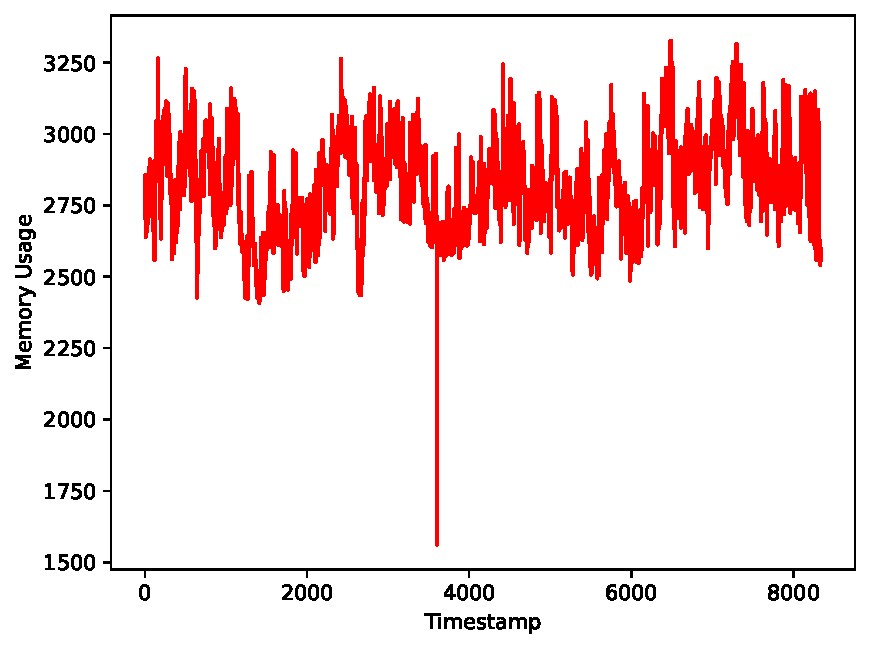
\includegraphics[width=0.49\linewidth]{/pdf/dataset/ram_full}
  \caption{Visualization of Google Trace CPU (left) and Google Trace RAM (right) datasets.} 
  \label{fig_data_ggtrace} 
\end{figure}
 
\subsubsection{EU Internet Traffic and UK Internet Traffic datasets}
	
	These two sets of data, which is used for experiments in \cite{cortez2012multi}, are recorded by two distinct ISPs. The EU Internet Traffic dataset comes from a private ISP playing a role as a reporter with centers  in 11 European cities. The data corresponds to a a transatlantic link and was collected from 06:57 hours on 7 June to 11:17 hours on 29 July 2005. The UK Internet Traffic is derived from m UKERNA and represents aggregated traffic in the United Kingdom academic network backbone. It was
reported between 19 November 2004, at 09:30
hours and 27 January 2005, at 11:11 hours. Both of two datasets are processed and summarized in every 5 minutes, creating EU Internet Traffic (14773 records) and UK Internet Traffic (19989 records) as the input in our experiments. 2D visualization of the data is shown in Fig. \ref{fig_data_it} as below.

\begin{figure}[!ht] 
   \centering
   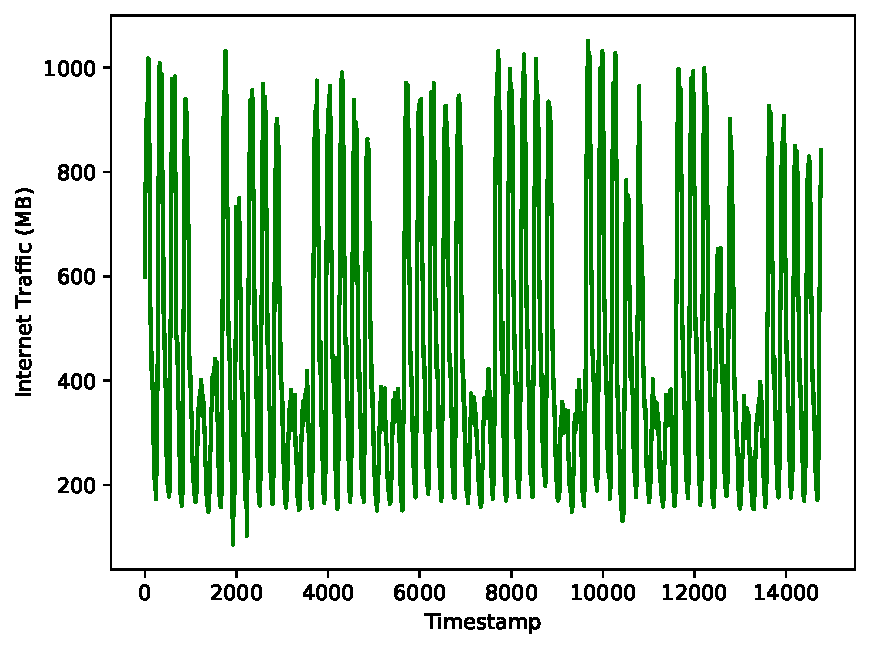
\includegraphics[width=0.49\linewidth]{/pdf/dataset/it_eu}
   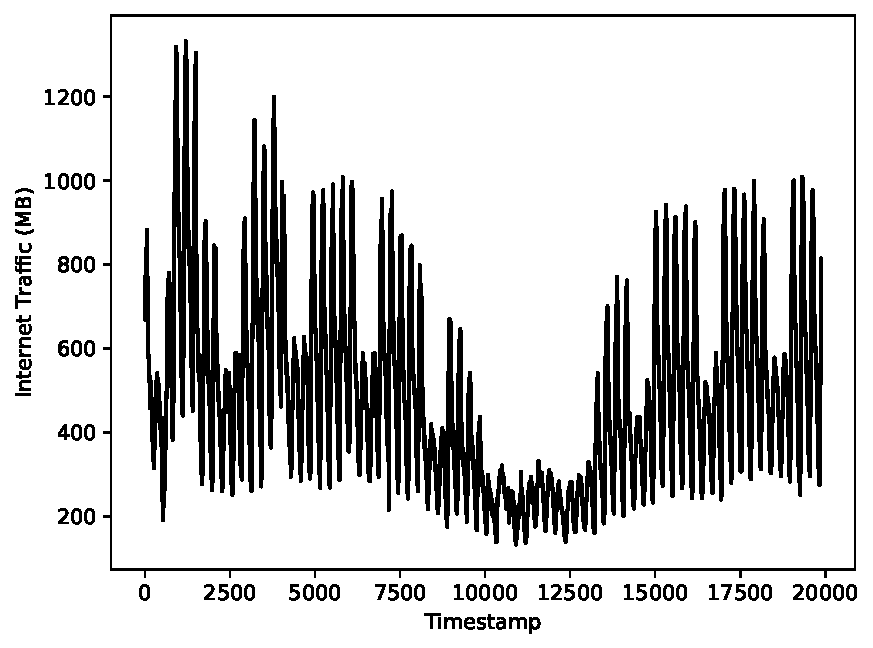
\includegraphics[width=0.49\linewidth]{/pdf/dataset/it_uk}
  \caption{Visualization of EU Internet Traffic (left) and UK Internet Traffic (right) datasets.} 
  \label{fig_data_it} 
\end{figure}

  

\subsection{Parameter Setting and Evaluation Metrics}
	
	As mentioned above, ISLO-CFNN's performance is compared with 4 deep learning models: MLPs, CFNN, LSTM and GRU, and 2 bio-inspired models: PSO-CFNN and SLnO-CFNN models. The hyper-parameter settings for each model are described as below:
\begin{itemize}
\item 4 datasets used for these experiments are all divided into 2 sets: training set and testing set with the ratio 0.8:0.2. The training set accounts for the first 80\% of the datasets, and the remaining is of testing set because of the sequential characteristic of time-series data.
\item CFNN's architectures in all models are configured with the same structure with three layers: input layer, one hidden layer and output layer which contains only one neuron in time-series prediction.
\item The input size for all models is 3 as we use 3 historical data points to predict the output in current time (mentioned in Section \ref{sec:application}).
\item RNN-based models as LSTM and GRU contains one input layer, LSTM (or GRU) blocks and one output layer with the same hyper-parameter setting as described in \cite{fu2016using}.
\item In all test, including with deep learning models and swarm-based algorithms, the number of iterations is set to 1000. From the experiments, we figure out that the amount of 1000 iterations is enough for all algorithms to converge to their final results. 
\end{itemize} 

Besides the common settings for models, the following settings are applied for each swarm-based algorithms as they show the best empirical performance:

\begin{itemize}
\item The population size for each algorithm is set to 200.
\item For PSO, based on the original paper \cite{eberhart1995particle}, cognitive learning rates $c_1=c_2=2.05$, and inertia factor $w$ is set linearly reducing from 0.9 to 0.4 over the course of iteration.
\item For SLnO and ISLO, hyper-parameters are set as described in original paper \cite{masadeh2019sea}, and also, $c_1$ and $c_2$ in ISLO algorithm are the same as shown for PSO.
\end{itemize}

\begin{table}[!t]
\caption{Comparision between models on each dataset by different measurements.}
\label{tbl_result_app}
\centering
\begin{tabular}{|l|l|l|l|l|}
\hline
Dataset                              & Model     & RMSE            & MAE             & MedAE          \\ \hline
\multirow{8}{*}{Google Trace CPU}    & CFNN      & \textbf{199.77} & 126.80          & 80.05          \\ \cline{2-5} 
                                     & FFNN      & 203.54          & 129.52          & 85.69          \\ \cline{2-5} 
                                     & LSTM      & 200.89          & 129.88          & 84.65          \\ \cline{2-5} 
                                     & GRU       & 201.88          & 130.50          & 82.96          \\ \cline{2-5} 
                                     & RNN       & \textbf{200.40} & 129.30          & 85.49          \\ \cline{2-5} 
                                     & PSO-CFNN  & 203.75          & 127.41          & 79.74          \\ \cline{2-5} 
                                     & SLnO-CFNN & 201.40          & \textbf{126.60} & \textbf{79.64} \\ \cline{2-5} 
                                     & ISLO-CFNN & 203.55          & \textbf{124.94} & \textbf{76.08} \\ \hline
\multirow{8}{*}{Google Trace RAM}    & CFNN      & 52.54           & 35.35           & 24.87          \\ \cline{2-5} 
                                     & FFNN      & 53.61           & 36.51           & 24.29          \\ \cline{2-5} 
                                     & LSTM      & 48.47           & 30.40           & 20.51          \\ \cline{2-5} 
                                     & GRU       & 48.43           & 30.74           & 20.78          \\ \cline{2-5} 
                                     & RNN       & \textbf{47.00}  & \textbf{28.86}  & \textbf{18.90} \\ \cline{2-5} 
                                     & PSO-CFNN  & 49.09           & 31.33           & 20.67          \\ \cline{2-5} 
                                     & SLnO-CFNN & 49.33           & 31.62           & 20.53          \\ \cline{2-5} 
                                     & ISLO-CFNN & \textbf{47.53}  & \textbf{29.80}  & \textbf{19.65} \\ \hline
\multirow{8}{*}{EU Internet Traffic} & CFNN      & \textbf{15.85}  & \textbf{11.30}  & \textbf{8.01}  \\ \cline{2-5} 
                                     & FFNN      & 16.48           & 11.79           & 8.41           \\ \cline{2-5} 
                                     & LSTM      & \textbf{15.84}  & \textbf{11.37}  & \textbf{8.30}  \\ \cline{2-5} 
                                     & GRU       & 17.39           & 13.09           & 10.29          \\ \cline{2-5} 
                                     & RNN       & 16.90           & 12.49           & 9.55           \\ \cline{2-5} 
                                     & PSO-CFNN  & 16.02           & 11.49           & 8.31           \\ \cline{2-5} 
                                     & SLnO-CFNN & 16.37           & 11.74           & 8.47           \\ \cline{2-5} 
                                     & ISLO-CFNN & 16.02           & 11.47           & 8.31           \\ \hline
\multirow{8}{*}{UK Internet Traffic} & CFNN      & 10.74           & 8.09            & 6.31           \\ \cline{2-5} 
                                     & FFNN      & 11.32           & 8.40            & 6.45           \\ \cline{2-5} 
                                     & LSTM      & \textbf{10.34}  & 7.65            & 5.85           \\ \cline{2-5} 
                                     & GRU       & 11.52           & 8.89            & 7.33           \\ \cline{2-5} 
                                     & RNN       & 11.27           & 8.38            & 6.39           \\ \cline{2-5} 
                                     & PSO-CFNN  & 10.43           & \textbf{7.59}   & \textbf{5.63}  \\ \cline{2-5} 
                                     & SLnO-CFNN & 10.61           & 7.73            & 5.75           \\ \cline{2-5} 
                                     & ISLO-CFNN & \textbf{10.46}  & \textbf{7.64}   & \textbf{5.77}  \\ \hline
\end{tabular}
\end{table}

	All 8 models' performance on 4 datasets are compared with each other in term of accuracy. In our experiments, mean absolute error (MAE) is used mainly for evaluation purposes. Beside MAE, root mean square error (RMSE) and median absolute error	(MedAE) are also used as measurements for comparision. These three measurement methods are very popular and widely used for evaluation in time-series prediction. Table. \ref{tbl_result_app} presents the results of all models on each dataset evaluated by MAE, RMSE and MedAE measurements. It is worth to mention here that the 2 best results on each evaluation measurement would be highlighted in bold. Also, Fig. \ref{fig_result_cpu_islo_rnn} illustrates the comparision between predicted output and the ground truth from ISLO-CFNN and RNN-based models running on Google Trace CPU dataset, while Fig. \ref{fig_result_ram} shows the performance of different optimizers including ISLO, SLnO, PSO and original Gradient Descent in optimizing CFNN parameters, running on Google Trace RAM dataset.



\subsection{Results and Discussion}  
\label{Results_app}
\subsubsection{Accuracy comparision}
	Table \ref{tbl_result_app} illustrates the comparision between ISLO-CFNN and other models on each dataset by different measurements. In general, ISLO-CFNN is very competitive in working on all dataset. Also, while ISLO provides good results in MAE and MedAE, RNN-based models (RNN, LSTM, GRU) and original CFNN show decent performance by giving the best RMSE.
	
\begin{figure}[!ht] 
   \centering
   	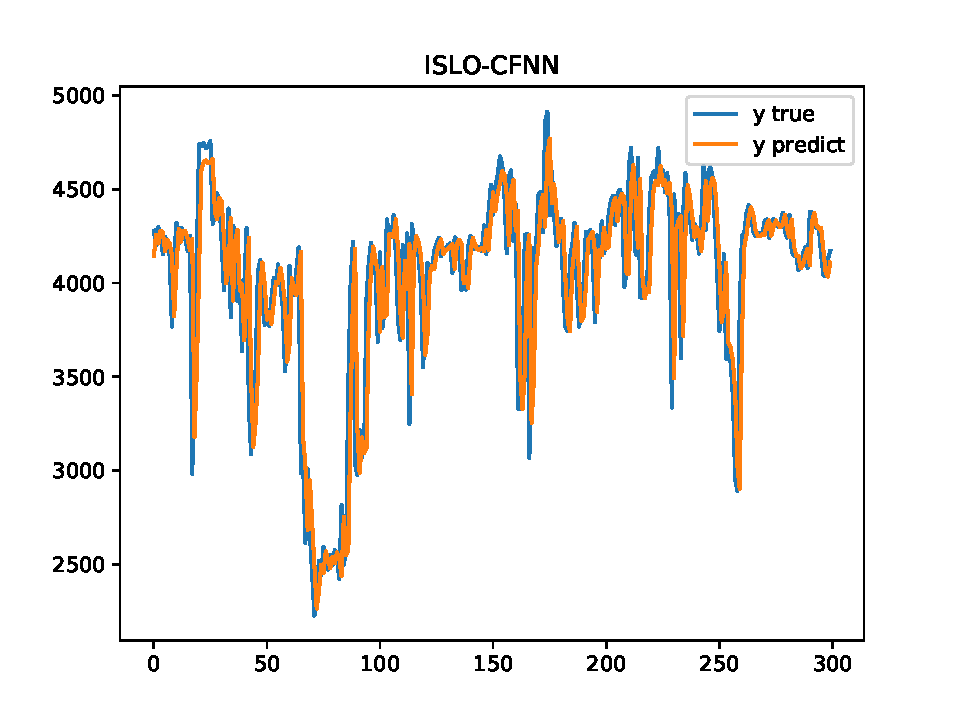
\includegraphics[width=0.49\linewidth]{pdf/result_data/cpu/ISLO_CFNN_cpu}
  	 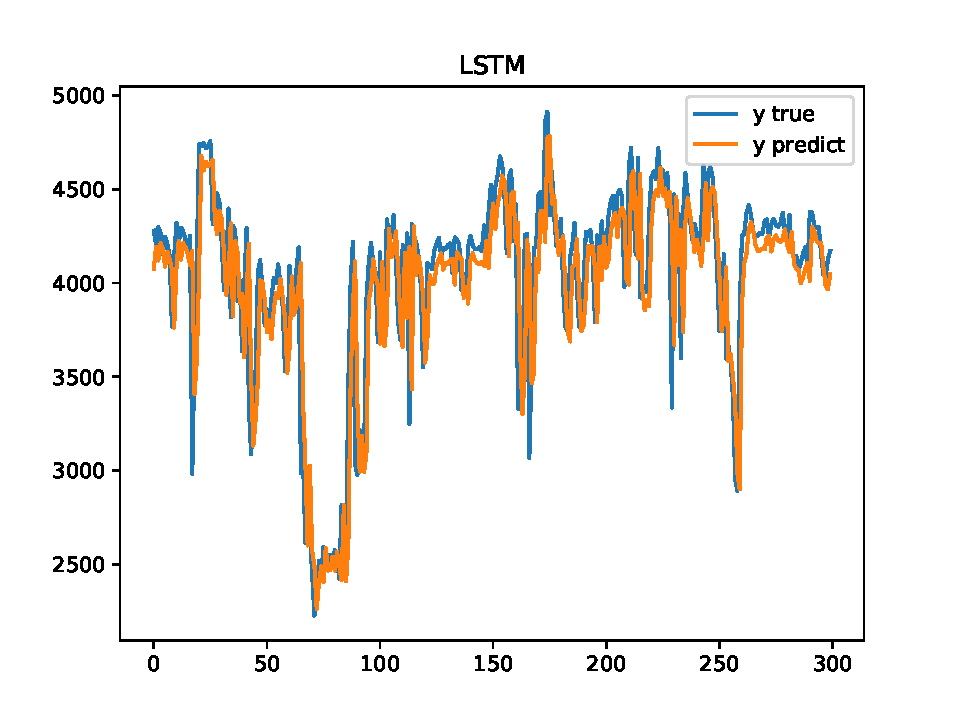
\includegraphics[width=0.49\linewidth]{pdf/result_data/cpu/LSTM_cpu}
  	 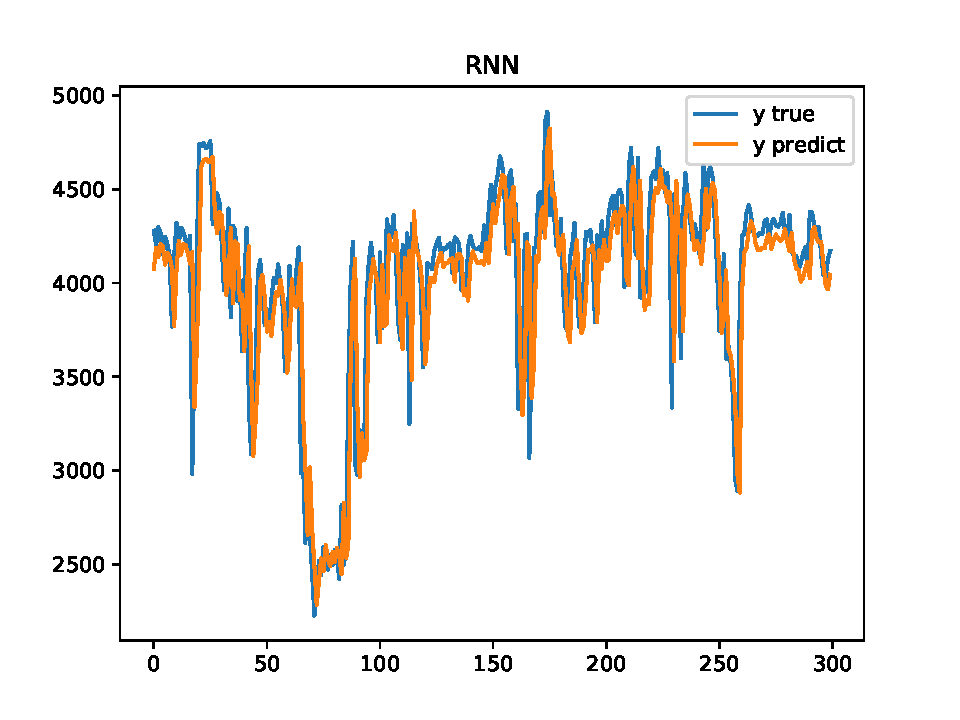
\includegraphics[width=0.49\linewidth]{pdf/result_data/cpu/RNN_cpu}
  	 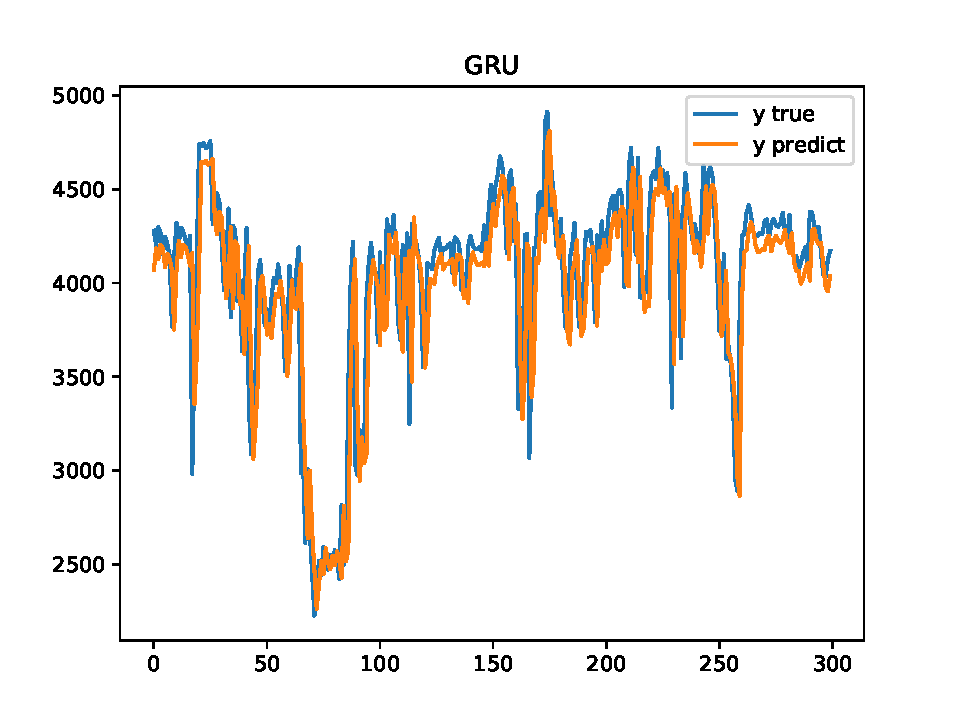
\includegraphics[width=0.49\linewidth]{pdf/result_data/cpu/GRU_cpu}
	
  \caption{Performance comparision between ISLO-CFNN and different recurrent-based deep learning models on Google Trace CPU data.} 
  \label{fig_result_cpu_islo_rnn} 
\end{figure}
	
	On Google Trace CPU dataset, ISLO-CFNN shows its outstanding performance, giving the best results in MAE and MedAE measurements. It is obvious that compared with RNN-based models, our CFNN-ISLO shows the superior performance, and provides better results (see Fig. \ref{fig_result_cpu_islo_rnn}). Specifically, the model's figures are better than LSTM by $3.9 \%$ (with MAE) and about $10 \%$ (with MedAE). CFNN and RNN provides the smallest RMSE on the dataset, while bio-inspred models including SLnO-CFNN and PSO-CFNN have advantages in MAE and MedAE.
	
\begin{figure}[!ht] 
   \centering
   	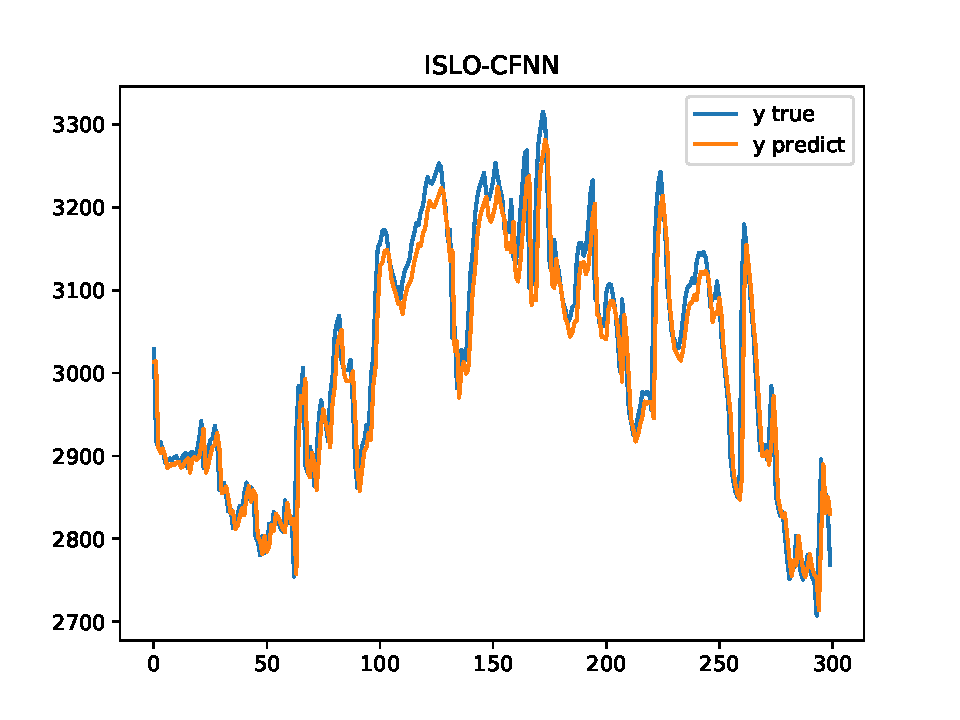
\includegraphics[width=0.49\linewidth]{pdf/result_data/ram/ISLO_CFNN_ram}
  	 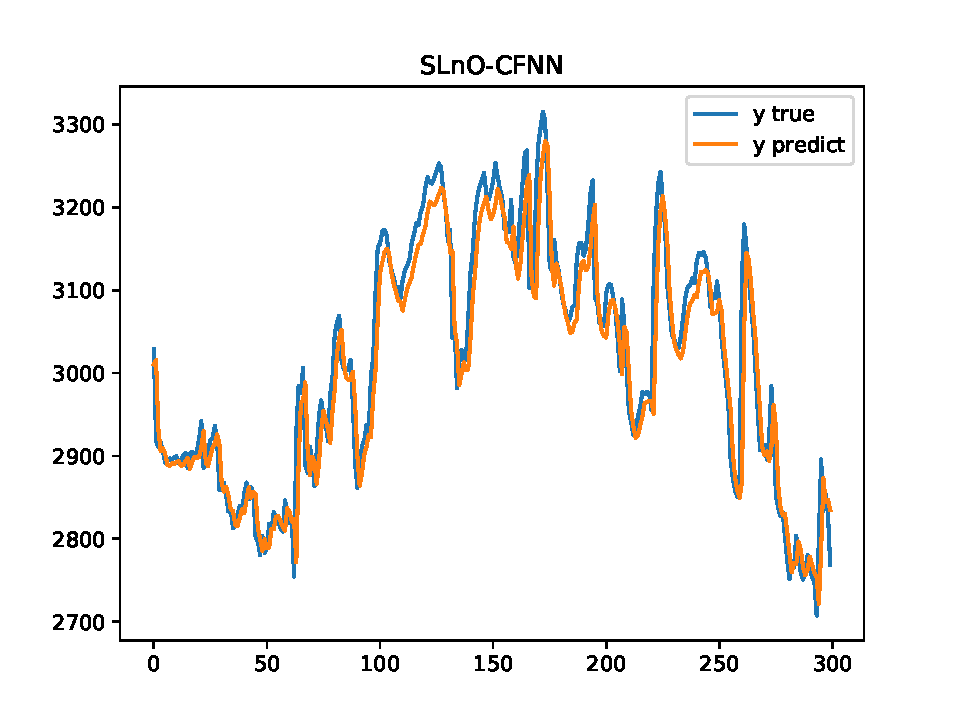
\includegraphics[width=0.49\linewidth]{pdf/result_data/ram/SLnO_CFNN_ram}
  	 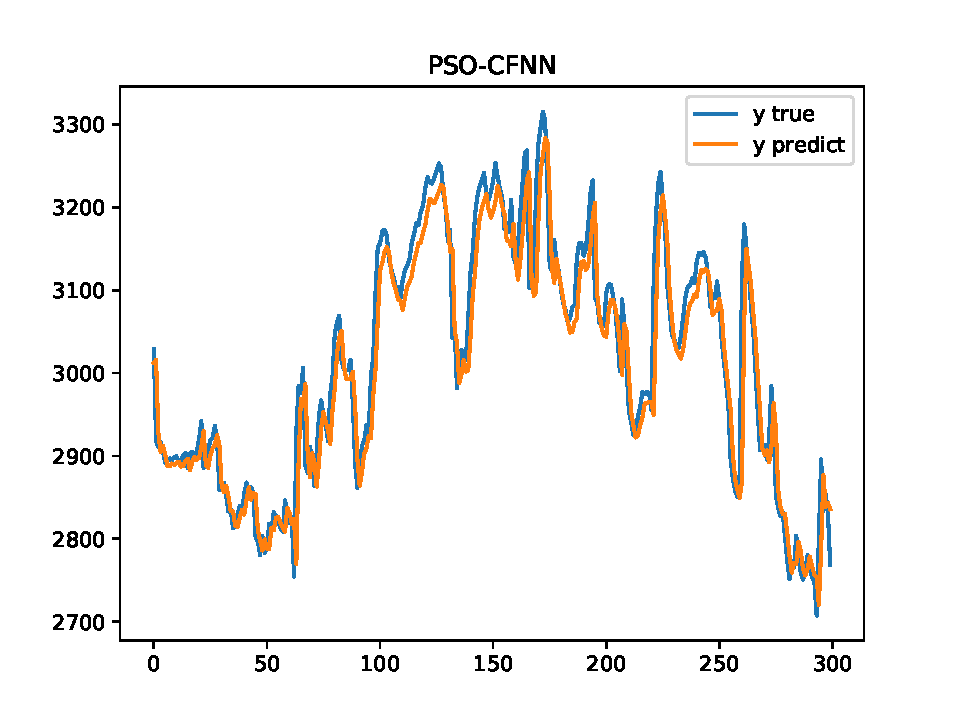
\includegraphics[width=0.49\linewidth]{pdf/result_data/ram/PSO_CFNN_ram}
  	 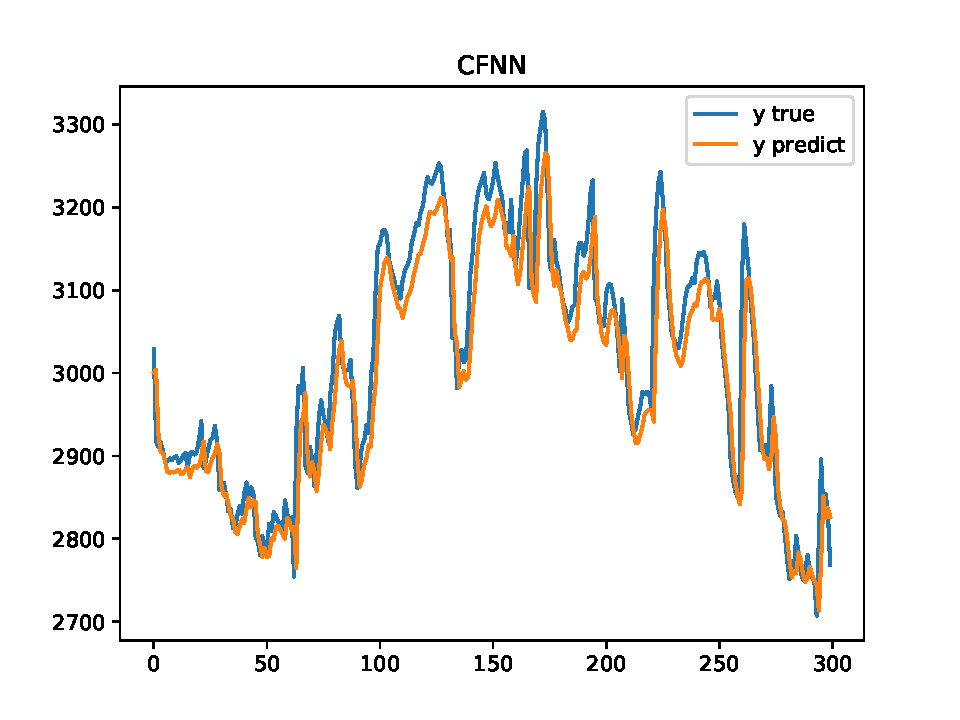
\includegraphics[width=0.49\linewidth]{pdf/result_data/ram/CFNN-1H_ram}
	
  \caption{Performance comparision between ISLO and other algorithms including Gradient Descent, PSO and SLnO on optimizing CFNN (Google Trace RAM data).} 
  \label{fig_result_ram} 
\end{figure}
	
	Working on Google Trace RAM and UK Internet Traffic datatsets, ISLO shows a competitive performance compared with the others, standing at the second position in terms of all measurements. ISLO-CFNN's results ony stand behind original RNN (Google Trace RAM) and PSO-CFNN (UK Internet Traffic). With Google Trace RAM dataset, ISLO-CFNN's performance is more superior than that of original CFNN by $9.6 \%$ (RMSE) and $16 \%$ (MAE), and with the others the model also show its prominence. Furthermore, Table \ref{tbl_result_app} shows that in both datasets, the gap between ISLO-CFNN's results and the best figures is trivial, proving that the model is able to work very well with them. It is worth mentioned here that compared with Gradient Descent, swarm-based optimization algorithms such as ISLO, SLnO and PSO show better performance on optimizing CFNN, working on Google Trace RAM data (see Fig. \ref{fig_result_ram})
	
	With the results illustarted in Table \ref{tbl_result_app} about EU Internet Traffic data, it is obvious that this is the data in which our model is less competitive than its performance on the other data. Original CFNN and LSTM provide the outstanding and mostly the same figures. Three swarm-based models including PSO-CFNN, ISLO-CFNN and SLnO-CFNN stand at right behind the best one, while GRU and RNN are much less competitive than the others.

\section{Chapter conclusion}
  In this chapter, we described our two experiments for testing the performance of ISLO algorithm as well as ISLO-CFNN model. The first experiment tests ISLO and other algrithms on optimizing 30 benchmark functions. The results show that ISLO outperforms most of compared algorithms in the majority of functions in terms of accuracy and robustness. The other experiment compares ISLO-CFNN performance with other well-known deep learning models and two other version of CFNN: SLnO-CFNN and PSO-CFNN, working on 4 datasets of workload. It is obvious that ISLO-CFNN provides very competitive results compared with the others in term of accuracy. Furthermore, ISLO and other swarm-based algorithms including PSO and SLnO shows better performance than the well-known BP algorithm when training CFNN model.
\end{document}